\chapter{Problema}

Da anni ormai si tenta di risolvere il problema del riconoscimento di testi contenuti in immagine. Il problema è noto come Optical Character Recognition (OCR) e consiste nel riconoscere i caratteri di un testo contenuto in un'immagine. Il problema è complesso e presenta una serie di insidie che non sono di immediata risoluzione. Nonostante ciò, allo stato dell'arte esistono diversi algoritmi che consentono di ottenere risultati soddisfacenti.
Quello che viene presentato in questo documento è un modello che mira a semplificare il problema a una sottoclasse di immagini, avendo il vantaggio di ottenere un algoritmo più leggero ed efficiente, a discapito della sua versatilità.

Capita spesso che le immagini da cui è utile estrarre il testo siano screenshot. L'algoritmo presentato si occupa di estrarre il testo contenuto in uno screenshot, indipendentemente dal font e dai colori utilizzati. Il problema viene semplificato ai font in stampatello e agli alfabeti italiano e latino esteso (punteggiatura compresa), escludendo il corsivo e altri alfabeti. Tramite l'uso di euristiche, si mostra come estendere l'implementazione per riconscere frasi (purché non siano divise su più righe), e non solo parole.

\begin{figure}[H]
	\centering
	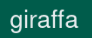
\includegraphics[width=0.3\textwidth]{images/giraffa.png}
	\caption{Screenshot di esempio}
	\label{fig:screenshot}
\end{figure}
